\documentclass{article}

\usepackage[german]{babel}
\usepackage{array}
\usepackage[letterpaper,top=2cm,bottom=2cm,left=3cm,right=3cm,marginparwidth=1.75cm]{geometry}

\usepackage{amsmath}
\usepackage{graphicx}
\usepackage{subcaption} % Added package
\usepackage[colorlinks=true, allcolors=blue]{hyperref}
\usepackage[T1]{fontenc}
\usepackage{tabularx}
\usepackage{booktabs}


\title{Übungsprotokoll - NWG2 - Übung 06 \\ Spanning Tree}
\author{\vspace{0.5cm} Thomas Brandstetter (s2210239002) \& Jakob Mayr (s2210239021)}

\begin{document}
\maketitle

\section{Konfiguration der Endsysteme}

In der folgenden Übung haben wir die PCs 4.1 und 4.2 benutzt, somit sind die Netze 4.x verwendet worden. Die IP-Konfiguration wird folgendermaßen vergeben: Klick auf „Network“ in der Taskleiste $\rightarrow$ „Network \& Internet Settings“ $\rightarrow$ „Change adapter options“ $\rightarrow$ gewünschtes Netzwerk Interface auswählen, in diesem Fall Ethernet 2 $\rightarrow$ „Properties“ $\rightarrow$ Doppelklick auf „Internet Protocol Version 4“ bzw. „Internet Protocol Version 6“. In den geöffneten Fenstern können wir nun jeweils die IP-Adresse, Subnetzmaske/Präfix und das Gateway eingeben (Bei dieser Übung benötigt es kein Default-Gateway, da alle Geräte im selben Netz sind). Folglich sind die Konfigurationen beider PCs zu sehen:

\begin{figure}[!htp]
  \centering
  \begin{minipage}[b]{0.45\textwidth}
    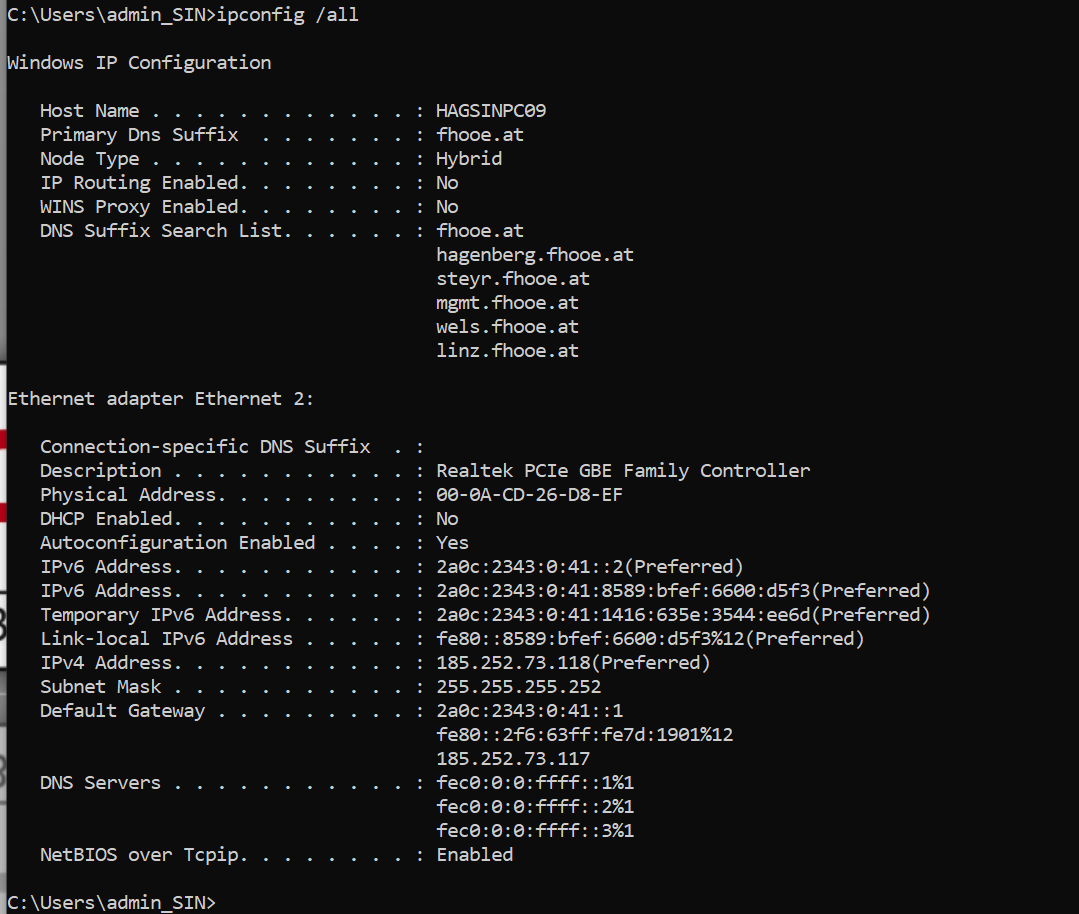
\includegraphics[width=\textwidth]{Arbeitsergebnisse/pc41/pc41_ipconfig.PNG}
    \caption{PC41 IPv4 und IPv6 config}
  \end{minipage}
  \hspace{0.8cm}
  \begin{minipage}[b]{0.45\textwidth}
    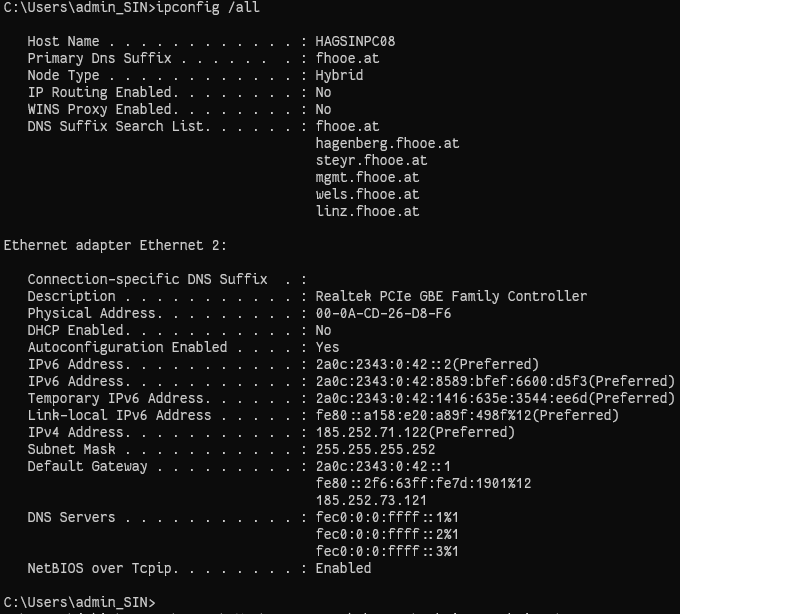
\includegraphics[width=\textwidth]{Arbeitsergebnisse/pc42/pc42_ipconfig.PNG}
    \caption{PC42 IPv4 und IPv6 config}
  \end{minipage}
\end{figure}

\pagebreak



\section{Konfiguration der Gruppenswitches}

\subsection{Konfigurieren der VLANs}

Auf den Switches wird sollen die VLANs 1 und 50 verwendet werden. VLAN 1 \\

\begin{table}[htbp]
    \centering
    \begin{tabularx}{\textwidth}{|X|X|}
        \toprule
        \textbf{Befehl} & \textbf{Erklärung} \\
        \midrule
        ... & ...\\
        \hline
        ... & ...\\
        \bottomrule
    \end{tabularx}
    \caption{Verwendete Befehle zur Konfiguration des Gruppenrouters}
\end{table}

\noindent notes...



\section{Konfiguration der Gruppenswitches}

...\\

\begin{table}[htbp]
    \centering
    \begin{tabularx}{\textwidth}{|X|X|}
        \toprule
        \textbf{Befehl} & \textbf{Erklärung} \\
        \midrule
        ... & ...\\
        \hline
        ... & ...\\
        \bottomrule
    \end{tabularx}
    \caption{Verwendete Befehle zur Konfiguration der Gruppenswitches}
    \label{tab:commands}
\end{table}
\noindent notes...

\section{Fragen zur Konfiguration}

\subsection*{Frage 6.1 \normalfont Warum muss das VLAN 1 nicht angelegt werden?}
Da es bereits existiert.\\

\subsection*{Frage 6.2 \normalfont Was ist die Funktion PortFast und wozu dient sie?}
...\\

\subsection*{Frage 6.3 \normalfont Als Root Bridge wird jene Switch verwendet, die die niederste Priority Nummer besitzt. Was passiert aber, wenn das nicht eindeutig ist?}
...\\

\subsection*{Frage 6.4 \normalfont Wie setzt sich der Priority Wert einer Brigde ID zusammen? Worauf muss bei der manuellen Vergabe geachtet werden?} 
...\\

\subsection*{Frage 6.5 \normalfont Wie unterscheidet sich das Verhalten von Rapid PVST vom nomralen PVST, und warum ist das der Fall?}
...\\

\pagebreak
\section{Tests und Interpretation ihrer Resultate}

\subsection{GS41 \& GS42}
Verwendete "Load-Balancing" Konfiguration auf des Switchtes GS41 und GS42:\\
\begin{figure}[!htp]
  \centering
  \begin{minipage}[b]{0.45\textwidth}
    \includegraphics[width=\textwidth]{Arbeitsergebnisse/GS41/GS41_etherchannel.png}
    \caption{GS41 EtherChannel Load-Balancing Configuration}
  \end{minipage}
  \hspace{0.8cm}
  \begin{minipage}[b]{0.45\textwidth}
    \includegraphics[width=\textwidth]{Arbeitsergebnisse/GS41/GS41_etherchannel.png}
    \caption{GS41 EtherChannel Load-Balancing Configuration}
  \end{minipage}
\end{figure}

\pagebreak
\subsection{PC41}
Ping von PC41 zu PC42, Ping zu Netz 8 - PC81 (fehlgeschlagen da ACL) und FTP-Verbindung\\
\begin{figure}[!htp]
  \centering
  \begin{minipage}[b]{0.25\textwidth}
    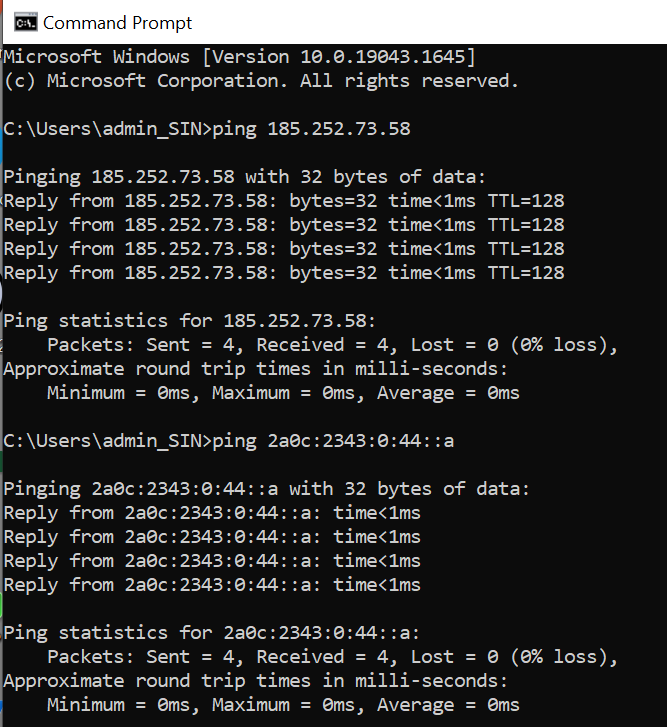
\includegraphics[width=\textwidth]{Arbeitsergebnisse/PC41/pc41_ping_pc42.png}
    \caption{PC41 ping PC42}
  \end{minipage}
  \hspace{0.8cm}
  \begin{minipage}[b]{0.25\textwidth}
    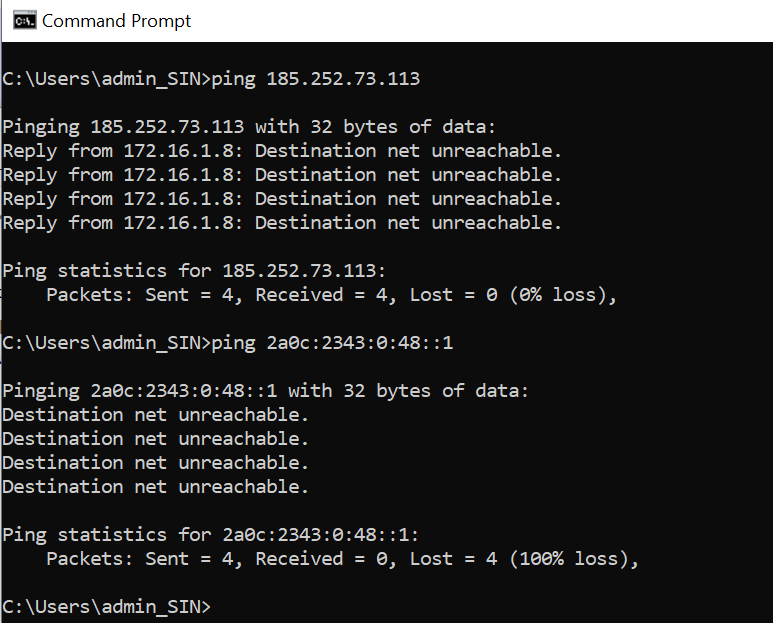
\includegraphics[width=\textwidth]{Arbeitsergebnisse/PC41/pc41_ping_failed.png}
    \caption{PC41 Ping zu Netz 8 - PC81 (fehlgeschlagen da ACL)}
  \end{minipage}
  \hspace{0.8cm}
  \begin{minipage}[b]{0.25\textwidth}
    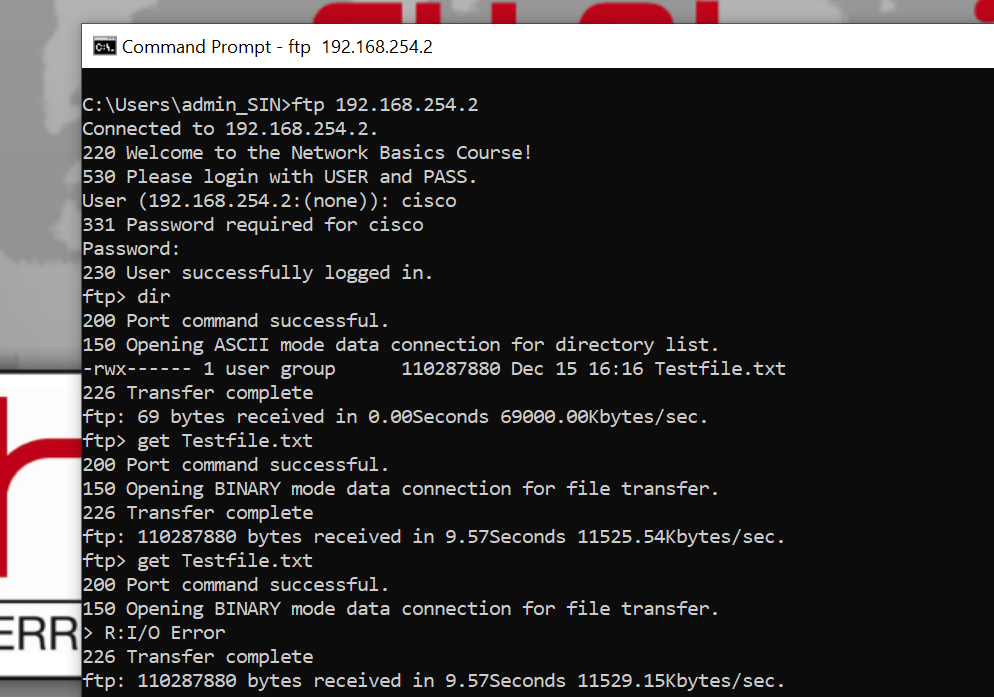
\includegraphics[width=\textwidth]{Arbeitsergebnisse/PC41/pc41_ftp.png}
    \caption{PC41 FTP-Verbindung}
  \end{minipage}
\end{figure}

\subsection{PC42}
Ping von PC42 zu PC41, Ping zu Netz 8 - PC82 (fehlgeschlagen da ACL) und FTP-Verbindung\\
\begin{figure}[!htp]
  \centering
  \begin{minipage}[b]{0.25\textwidth}
    \includegraphics[width=\textwidth]{Arbeitsergebnisse/PC42/pc42_ping_PC41.png}
    \caption{PC42 ping PC41}
  \end{minipage}
  \hspace{0.8cm}
  \begin{minipage}[b]{0.25\textwidth}
    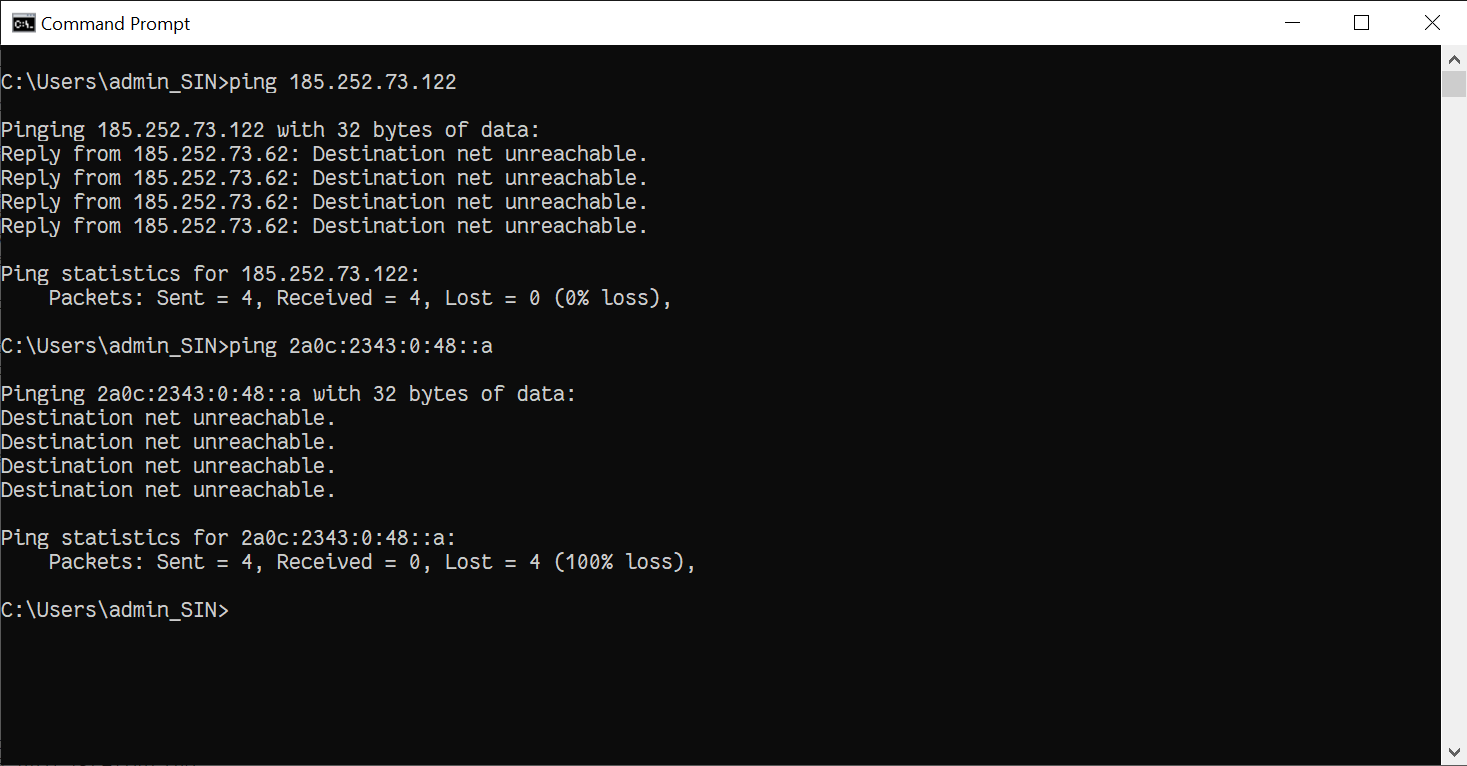
\includegraphics[width=\textwidth]{Arbeitsergebnisse/PC42/pc42_ping_failed.png}
    \caption{PC42 Ping zu Netz 8 - PC82 (fehlgeschlagen da ACL)}
  \end{minipage}
  \hspace{0.8cm}
  \begin{minipage}[b]{0.25\textwidth}
    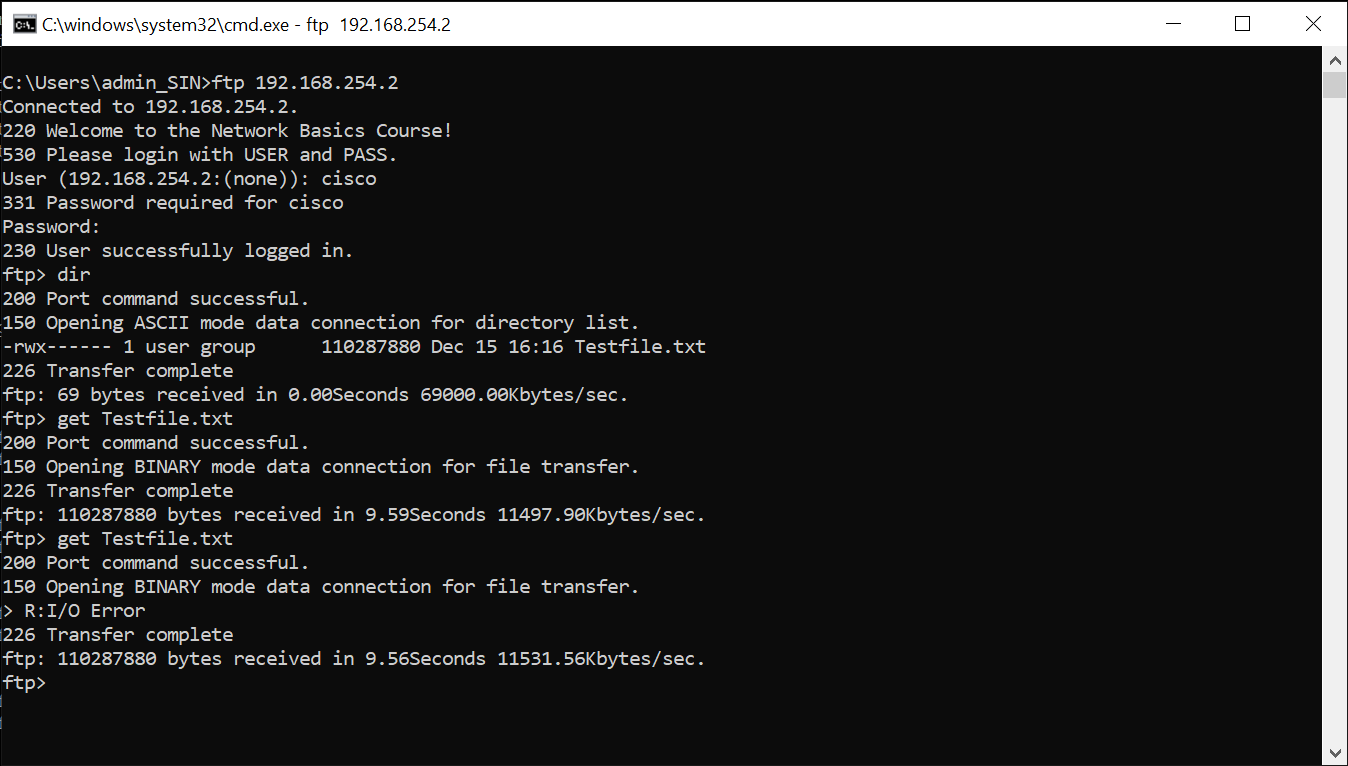
\includegraphics[width=\textwidth]{Arbeitsergebnisse/PC42/pc42_ftp.png}
    \caption{PC42 FTP-Verbindung}
  \end{minipage}
\end{figure}

\end{document}

